\chapter{Week}
\begin{figure}[!htb]
	\centering
		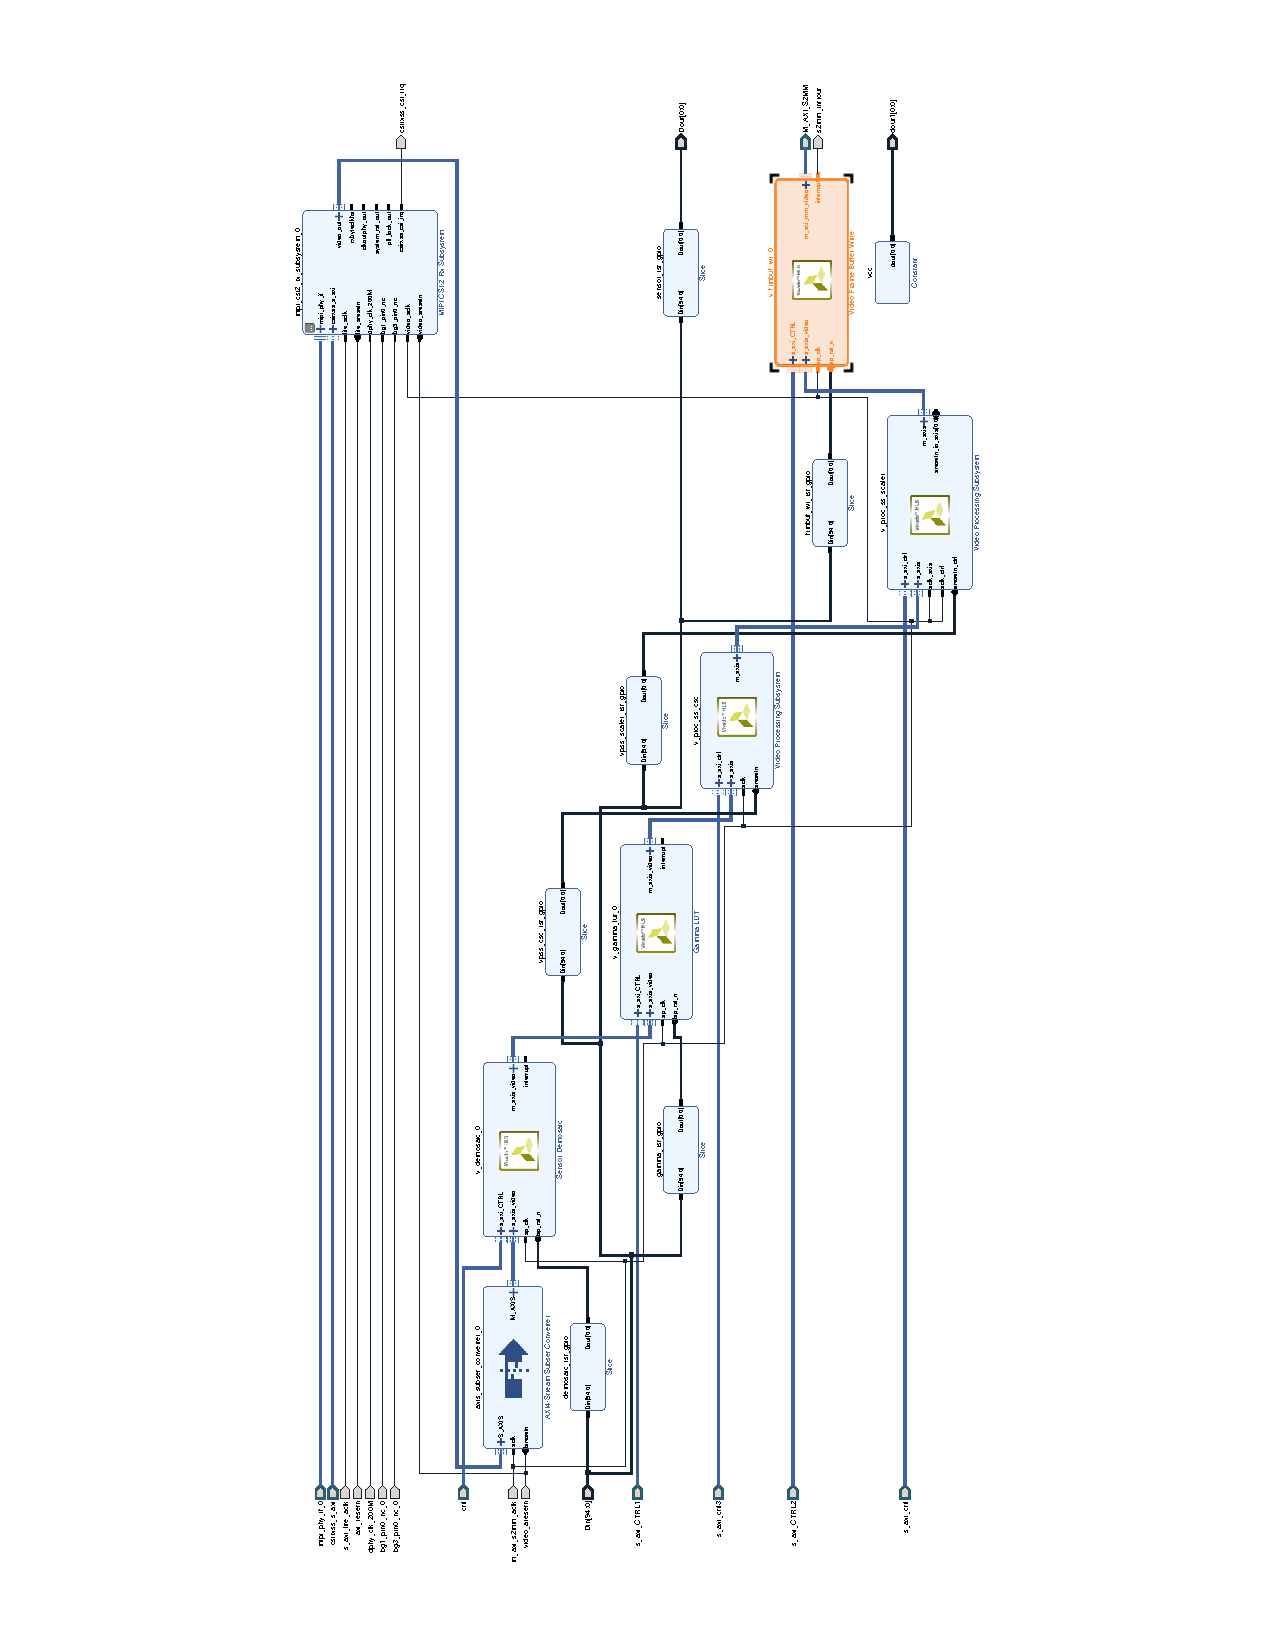
\includegraphics[width=\textwidth]{bilder/mipi_csi2_rx.pdf}
		\caption{\acs{MIPI} \acs{CSI} block design}
		\label{fig:mipi_block}
\end{figure}
Figure~\ref{fig:mipi_block} shows the reference design provided by Xilinx for the ZCU 104 board showing the complete hierarchy of the \ac{MIPI} \ac{CSI} block design with all additional blocks. These blocks are needed for further image processing. The data coming from the image sensor is in an unprocessed format called RAW. Therefore, an image processing pipeline needs to be integrated to convert this RAW image format into useable data in RGB format for example. The following Xilinx \acp{IP} are used to accomplish this task: 'Sensor Demosaic', 'Gamma LUT', 'Video Processing subsystem' and 'Video Frame Buffer Write'. The data transfer is handled by \ac{AXI} streaming interfaces.
Using the reference design as a starting point, the \ac{MIPI} subsystem was integrated into the hardware design together with the \ac{DPU} block. Afterward, Petalinux had to be configured and built. This enabled control of the whole system via an embedded Linux \ac{OS} host system running on the ARM cores. Several steps are necessary for setting up a Petalinux environment:
\begin{itemize}
	\item \textbf{Vivado hardware design:} First of all a working hardware design needed to be created in Vivado and successfully synthesized. This hardware design then needs to be exported in .hdf file format. This allows importing the hardware design as a template for the Petalinux system generation.
	\item \textbf{Creation of Petalinux project:} Petalinux is a command line tool for a Linux \ac{OS} which abstracts away some of the details of building an embedded Linux \ac{OS}. During generation of a new project, the previously used hardware design file is imported so that the system can access all of the implemented features.
	\item \textbf{Configuration:} In the next steps, necessary packages, user written apps, file system packages and custom modules can be added to the Petalinux project via console commands and a \ac{GUI} environment simplifying interaction with all of the possible options.
	\item \textbf{Building the system:} After all of the system is configured, the necessary packages and files need to be downloaded and a root file system and kernel image constructed. This can also be done via console commands. After successfully building the whole system the necessary files need to be generated for the system to boot. This includes a BOOT.bin file, an image.ub file and the root file system. These files and directories are the minimum necessities for the Petalinux \ac{OS}
\end{itemize}
To create a bootable image, an SD card is used and properly formatted. The SD card needs to partitioned into two primary partitions, BOOT formatted as FAT32 and ROOTFS, formatted as ext4. The Petalinux files are then copied over into the respective directories and the SD card can be used as the boot image for the \ac{FPGA} board.
Another Synthara conference call was due to further discuss details about the Embedded World 2019 demonstrator and a visit was organized to the company in order to create a schedule for the collaboration and labor division between Enclustra and Synthara.